
%% bare_adv.tex
%% V1.4a
%% 2014/09/17
%% by Michael Shell
%% See: 
%% http://www.michaelshell.org/
%% for current contact information.
%%
%% This is a skeleton file demonstrating the advanced use of IEEEtran.cls
%% (requires IEEEtran.cls version 1.8a or later) with an IEEE Computer
%% Society journal paper.
%%
%% Support sites:
%% http://www.michaelshell.org/tex/ieeetran/
%% http://www.ctan.org/tex-archive/macros/latex/contrib/IEEEtran/
%% and
%% http://www.ieee.org/

%%*************************************************************************
%% Legal Notice:
%% This code is offered as-is without any warranty either expressed or
%% implied; without even the implied warranty of MERCHANTABILITY or
%% FITNESS FOR A PARTICULAR PURPOSE! 
%% User assumes all risk.
%% In no event shall IEEE or any contributor to this code be liable for
%% any damages or losses, including, but not limited to, incidental,
%% consequential, or any other damages, resulting from the use or misuse
%% of any information contained here.
%%
%% All comments are the opinions of their respective authors and are not
%% necessarily endorsed by the IEEE.
%%
%% This work is distributed under the LaTeX Project Public License (LPPL)
%% ( http://www.latex-project.org/ ) version 1.3, and may be freely used,
%% distributed and modified. A copy of the LPPL, version 1.3, is included
%% in the base LaTeX documentation of all distributions of LaTeX released
%% 2003/12/01 or later.
%% Retain all contribution notices and credits.
%% ** Modified files should be clearly indicated as such, including  **
%% ** renaming them and changing author support contact information. **
%%
%% File list of work: IEEEtran.cls, IEEEtran_HOWTO.pdf, bare_adv.tex,
%%                    bare_conf.tex, bare_jrnl.tex, bare_conf_compsoc.tex,
%%                    bare_jrnl_compsoc.tex, bare_jrnl_transmag.tex
%%*************************************************************************


% *** Authors should verify (and, if needed, correct) their LaTeX system  ***
% *** with the testflow diagnostic prior to trusting their LaTeX platform ***
% *** with production work. IEEE's font choices and paper sizes can       ***
% *** trigger bugs that do not appear when using other class files.       ***                          ***
% The testflow support page is at:
% http://www.michaelshell.org/tex/testflow/


% IEEEtran V1.7 and later provides for these CLASSINPUT macros to allow the
% user to reprogram some IEEEtran.cls defaults if needed. These settings
% override the internal defaults of IEEEtran.cls regardless of which class
% options are used. Do not use these unless you have good reason to do so as
% they can result in nonIEEE compliant documents. User beware. ;)
%
%\newcommand{\CLASSINPUTbaselinestretch}{1.0} % baselinestretch
%\newcommand{\CLASSINPUTinnersidemargin}{1in} % inner side margin
%\newcommand{\CLASSINPUToutersidemargin}{1in} % outer side margin
%\newcommand{\CLASSINPUTtoptextmargin}{1in}   % top text margin
%\newcommand{\CLASSINPUTbottomtextmargin}{1in}% bottom text margin




%
\documentclass[10pt,journal,compsoc]{IEEEtran}
% If IEEEtran.cls has not been installed into the LaTeX system files,
% manually specify the path to it like:
% \documentclass[10pt,journal,compsoc]{../sty/IEEEtran}


% For Computer Society journals, IEEEtran defaults to the use of 
% Palatino/Palladio as is done in IEEE Computer Society journals.
% To go back to Times Roman, you can use this code:
%\renewcommand{\rmdefault}{ptm}\selectfont





% Some very useful LaTeX packages include:
% (uncomment the ones you want to load)



% *** MISC UTILITY PACKAGES ***
%
%\usepackage{ifpdf}
% Heiko Oberdiek's ifpdf.sty is very useful if you need conditional
% compilation based on whether the output is pdf or dvi.
% usage:
% \ifpdf
%   % pdf code
% \else
%   % dvi code
% \fi
% The latest version of ifpdf.sty can be obtained from:
% http://www.ctan.org/tex-archive/macros/latex/contrib/oberdiek/
% Also, note that IEEEtran.cls V1.7 and later provides a builtin
% \ifCLASSINFOpdf conditional that works the same way.
% When switching from latex to pdflatex and vice-versa, the compiler may
% have to be run twice to clear warning/error messages.


%\usepackage{float}



% *** CITATION PACKAGES ***
%
\ifCLASSOPTIONcompsoc
  % IEEE Computer Society needs nocompress option
  % requires cite.sty v4.0 or later (November 2003)
  \usepackage[nocompress]{cite}
\else
  % normal IEEE
  \usepackage{cite}
\fi
% cite.sty was written by Donald Arseneau
% V1.6 and later of IEEEtran pre-defines the format of the cite.sty package
% \cite{} output to follow that of IEEE. Loading the cite package will
% result in citation numbers being automatically sorted and properly
% "compressed/ranged". e.g., [1], [9], [2], [7], [5], [6] without using
% cite.sty will become [1], [2], [5]--[7], [9] using cite.sty. cite.sty's
% \cite will automatically add leading space, if needed. Use cite.sty's
% noadjust option (cite.sty V3.8 and later) if you want to turn this off
% such as if a citation ever needs to be enclosed in parenthesis.
% cite.sty is already installed on most LaTeX systems. Be sure and use
% version 5.0 (2009-03-20) and later if using hyperref.sty.
% The latest version can be obtained at:
% http://www.ctan.org/tex-archive/macros/latex/contrib/cite/
% The documentation is contained in the cite.sty file itself.
%
% Note that some packages require special options to format as the Computer
% Society requires. In particular, Computer Society  papers do not use
% compressed citation ranges as is done in typical IEEE papers
% (e.g., [1]-[4]). Instead, they list every citation separately in order
% (e.g., [1], [2], [3], [4]). To get the latter we need to load the cite
% package with the nocompress option which is supported by cite.sty v4.0
% and later.





% *** GRAPHICS RELATED PACKAGES ***
%
\ifCLASSINFOpdf
  \usepackage[pdftex]{graphicx}
  % declare the path(s) where your graphic files are
  % \graphicspath{{../pdf/}{../jpeg/}}
  % and their extensions so you won't have to specify these with
  % every instance of \includegraphics
  % \DeclareGraphicsExtensions{.pdf,.jpeg,.png}
\else
  % or other class option (dvipsone, dvipdf, if not using dvips). graphicx
  % will default to the driver specified in the system graphics.cfg if no
  % driver is specified.
  % \usepackage[dvips]{graphicx}
  % declare the path(s) where your graphic files are
  % \graphicspath{{../eps/}}
  % and their extensions so you won't have to specify these with
  % every instance of \includegraphics
  % \DeclareGraphicsExtensions{.eps}
\fi
% graphicx was written by David Carlisle and Sebastian Rahtz. It is
% required if you want graphics, photos, etc. graphicx.sty is already
% installed on most LaTeX systems. The latest version and documentation
% can be obtained at: 
% http://www.ctan.org/tex-archive/macros/latex/required/graphics/
% Another good source of documentation is "Using Imported Graphics in
% LaTeX2e" by Keith Reckdahl which can be found at:
% http://www.ctan.org/tex-archive/info/epslatex/
%
% latex, and pdflatex in dvi mode, support graphics in encapsulated
% postscript (.eps) format. pdflatex in pdf mode supports graphics
% in .pdf, .jpeg, .png and .mps (metapost) formats. Users should ensure
% that all non-photo figures use a vector format (.eps, .pdf, .mps) and
% not a bitmapped formats (.jpeg, .png). IEEE frowns on bitmapped formats
% which can result in "jaggedy"/blurry rendering of lines and letters as
% well as large increases in file sizes.
%
% You can find documentation about the pdfTeX application at:
% http://www.tug.org/applications/pdftex





% *** MATH PACKAGES ***
%
%\usepackage[cmex10]{amsmath}
% A popular package from the American Mathematical Society that provides
% many useful and powerful commands for dealing with mathematics. If using
% it, be sure to load this package with the cmex10 option to ensure that
% only type 1 fonts will utilized at all point sizes. Without this option,
% it is possible that some math symbols, particularly those within
% footnotes, will be rendered in bitmap form which will result in a
% document that can not be IEEE Xplore compliant!
%
% Also, note that the amsmath package sets \interdisplaylinepenalty to 10000
% thus preventing page breaks from occurring within multiline equations. Use:
%\interdisplaylinepenalty=2500
% after loading amsmath to restore such page breaks as IEEEtran.cls normally
% does. amsmath.sty is already installed on most LaTeX systems. The latest
% version and documentation can be obtained at:
% http://www.ctan.org/tex-archive/macros/latex/required/amslatex/math/





% *** SPECIALIZED LIST PACKAGES ***
%\usepackage{acronym}
% acronym.sty was written by Tobias Oetiker. This package provides tools for
% managing documents with large numbers of acronyms. (You don't *have* to
% use this package - unless you have a lot of acronyms, you may feel that
% such package management of them is bit of an overkill.)
% Do note that the acronym environment (which lists acronyms) will have a
% problem when used under IEEEtran.cls because acronym.sty relies on the
% description list environment - which IEEEtran.cls has customized for
% producing IEEE style lists. A workaround is to declared the longest
% label width via the IEEEtran.cls \IEEEiedlistdecl global control:
%
% \renewcommand{\IEEEiedlistdecl}{\IEEEsetlabelwidth{SONET}}
% \begin{acronym}
%
% \end{acronym}
% \renewcommand{\IEEEiedlistdecl}{\relax}% remember to reset \IEEEiedlistdecl
%
% instead of using the acronym environment's optional argument.
% The latest version and documentation can be obtained at:
% http://www.ctan.org/tex-archive/macros/latex/contrib/acronym/


%\usepackage{algorithmic}
% algorithmic.sty was written by Peter Williams and Rogerio Brito.
% This package provides an algorithmic environment fo describing algorithms.
% You can use the algorithmic environment in-text or within a figure
% environment to provide for a floating algorithm. Do NOT use the algorithm
% floating environment provided by algorithm.sty (by the same authors) or
% algorithm2e.sty (by Christophe Fiorio) as IEEE does not use dedicated
% algorithm float types and packages that provide these will not provide
% correct IEEE style captions. The latest version and documentation of
% algorithmic.sty can be obtained at:
% http://www.ctan.org/tex-archive/macros/latex/contrib/algorithms/
% There is also a support site at:
% http://algorithms.berlios.de/index.html
% Also of interest may be the (relatively newer and more customizable)
% algorithmicx.sty package by Szasz Janos:
% http://www.ctan.org/tex-archive/macros/latex/contrib/algorithmicx/




% *** ALIGNMENT PACKAGES ***
%
%\usepackage{array}
% Frank Mittelbach's and David Carlisle's array.sty patches and improves
% the standard LaTeX2e array and tabular environments to provide better
% appearance and additional user controls. As the default LaTeX2e table
% generation code is lacking to the point of almost being broken with
% respect to the quality of the end results, all users are strongly
% advised to use an enhanced (at the very least that provided by array.sty)
% set of table tools. array.sty is already installed on most systems. The
% latest version and documentation can be obtained at:
% http://www.ctan.org/tex-archive/macros/latex/required/tools/


%\usepackage{mdwmath}
%\usepackage{mdwtab}
% Also highly recommended is Mark Wooding's extremely powerful MDW tools,
% especially mdwmath.sty and mdwtab.sty which are used to format equations
% and tables, respectively. The MDWtools set is already installed on most
% LaTeX systems. The lastest version and documentation is available at:
% http://www.ctan.org/tex-archive/macros/latex/contrib/mdwtools/


% IEEEtran contains the IEEEeqnarray family of commands that can be used to
% generate multiline equations as well as matrices, tables, etc., of high
% quality.


%\usepackage{eqparbox}
% Also of notable interest is Scott Pakin's eqparbox package for creating
% (automatically sized) equal width boxes - aka "natural width parboxes".
% Available at:
% http://www.ctan.org/tex-archive/macros/latex/contrib/eqparbox/




% *** SUBFIGURE PACKAGES ***
%\ifCLASSOPTIONcompsoc
%  \usepackage[caption=false,font=footnotesize,labelfont=sf,textfont=sf]{subfig}
%\else
%  \usepackage[caption=false,font=footnotesize]{subfig}
%\fi
% subfig.sty, written by Steven Douglas Cochran, is the modern replacement
% for subfigure.sty, the latter of which is no longer maintained and is
% incompatible with some LaTeX packages including fixltx2e. However,
% subfig.sty requires and automatically loads Axel Sommerfeldt's caption.sty
% which will override IEEEtran.cls' handling of captions and this will result
% in non-IEEE style figure/table captions. To prevent this problem, be sure
% and invoke subfig.sty's "caption=false" package option (available since
% subfig.sty version 1.3, 2005/06/28) as this is will preserve IEEEtran.cls
% handling of captions.
% Note that the Computer Society format requires a sans serif font rather
% than the serif font used in traditional IEEE formatting and thus the need
% to invoke different subfig.sty package options depending on whether
% compsoc mode has been enabled.
%
% The latest version and documentation of subfig.sty can be obtained at:
% http://www.ctan.org/tex-archive/macros/latex/contrib/subfig/




% *** FLOAT PACKAGES ***
%
%\usepackage{fixltx2e}
% fixltx2e, the successor to the earlier fix2col.sty, was written by
% Frank Mittelbach and David Carlisle. This package corrects a few problems
% in the LaTeX2e kernel, the most notable of which is that in current
% LaTeX2e releases, the ordering of single and double column floats is not
% guaranteed to be preserved. Thus, an unpatched LaTeX2e can allow a
% single column figure to be placed prior to an earlier double column
% figure. The latest version and documentation can be found at:
% http://www.ctan.org/tex-archive/macros/latex/base/

%\usepackage{stfloats}
% stfloats.sty was written by Sigitas Tolusis. This package gives LaTeX2e
% the ability to do double column floats at the bottom of the page as well
% as the top. (e.g., "\begin{figure*}[!b]" is not normally possible in
% LaTeX2e). It also provides a command:
%\fnbelowfloat
% to enable the placement of footnotes below bottom floats (the standard
% LaTeX2e kernel puts them above bottom floats). This is an invasive package
% which rewrites many portions of the LaTeX2e float routines. It may not work
% with other packages that modify the LaTeX2e float routines. The latest
% version and documentation can be obtained at:
% http://www.ctan.org/tex-archive/macros/latex/contrib/sttools/
% Do not use the stfloats baselinefloat ability as IEEE does not allow
% \baselineskip to stretch. Authors submitting work to the IEEE should note
% that IEEE rarely uses double column equations and that authors should try
% to avoid such use. Do not be tempted to use the cuted.sty or midfloat.sty
% packages (also by Sigitas Tolusis) as IEEE does not format its papers in
% such ways.
% Do not attempt to use stfloats with fixltx2e as they are incompatible.
% Instead, use Morten Hogholm'a dblfloatfix which combines the features
% of both fixltx2e and stfloats:
%
% \usepackage{dblfloatfix}
% The latest version can be found at:
% http://www.ctan.org/tex-archive/macros/latex/contrib/dblfloatfix/


%\ifCLASSOPTIONcaptionsoff
%  \usepackage[nomarkers]{endfloat}
% \let\MYoriglatexcaption\caption
% \renewcommand{\caption}[2][\relax]{\MYoriglatexcaption[#2]{#2}}
%\fi
% endfloat.sty was written by James Darrell McCauley, Jeff Goldberg and 
% Axel Sommerfeldt. This package may be useful when used in conjunction with 
% IEEEtran.cls'  captionsoff option. Some IEEE journals/societies require that
% submissions have lists of figures/tables at the end of the paper and that
% figures/tables without any captions are placed on a page by themselves at
% the end of the document. If needed, the draftcls IEEEtran class option or
% \CLASSINPUTbaselinestretch interface can be used to increase the line
% spacing as well. Be sure and use the nomarkers option of endfloat to
% prevent endfloat from "marking" where the figures would have been placed
% in the text. The two hack lines of code above are a slight modification of
% that suggested by in the endfloat docs (section 8.4.1) to ensure that
% the full captions always appear in the list of figures/tables - even if
% the user used the short optional argument of \caption[]{}.
% IEEE papers do not typically make use of \caption[]'s optional argument,
% so this should not be an issue. A similar trick can be used to disable
% captions of packages such as subfig.sty that lack options to turn off
% the subcaptions:
% For subfig.sty:
% \let\MYorigsubfloat\subfloat
% \renewcommand{\subfloat}[2][\relax]{\MYorigsubfloat[]{#2}}
% However, the above trick will not work if both optional arguments of
% the \subfloat command are used. Furthermore, there needs to be a
% description of each subfigure *somewhere* and endfloat does not add
% subfigure captions to its list of figures. Thus, the best approach is to
% avoid the use of subfigure captions (many IEEE journals avoid them anyway)
% and instead reference/explain all the subfigures within the main caption.
% The latest version of endfloat.sty and its documentation can obtained at:
% http://www.ctan.org/tex-archive/macros/latex/contrib/endfloat/
%
% The IEEEtran \ifCLASSOPTIONcaptionsoff conditional can also be used
% later in the document, say, to conditionally put the References on a 
% page by themselves.





% *** PDF, URL AND HYPERLINK PACKAGES ***
%
\usepackage{url}
% url.sty was written by Donald Arseneau. It provides better support for
% handling and breaking URLs. url.sty is already installed on most LaTeX
% systems. The latest version and documentation can be obtained at:
% http://www.ctan.org/tex-archive/macros/latex/contrib/url/
% Basically, \url{my_url_here}.


% NOTE: PDF thumbnail features are not required in IEEE papers
%       and their use requires extra complexity and work.
%\ifCLASSINFOpdf
%  \usepackage[pdftex]{thumbpdf}
%\else
%  \usepackage[dvips]{thumbpdf}
%\fi
% thumbpdf.sty and its companion Perl utility were written by Heiko Oberdiek.
% It allows the user a way to produce PDF documents that contain fancy
% thumbnail images of each of the pages (which tools like acrobat reader can
% utilize). This is possible even when using dvi->ps->pdf workflow if the
% correct thumbpdf driver options are used. thumbpdf.sty incorporates the
% file containing the PDF thumbnail information (filename.tpm is used with
% dvips, filename.tpt is used with pdftex, where filename is the base name of
% your tex document) into the final ps or pdf output document. An external
% utility, the thumbpdf *Perl script* is needed to make these .tpm or .tpt
% thumbnail files from a .ps or .pdf version of the document (which obviously
% does not yet contain pdf thumbnails). Thus, one does a:
% 
% thumbpdf filename.pdf 
%
% to make a filename.tpt, and:
%
% thumbpdf --mode dvips filename.ps
%
% to make a filename.tpm which will then be loaded into the document by
% thumbpdf.sty the NEXT time the document is compiled (by pdflatex or
% latex->dvips->ps2pdf). Users must be careful to regenerate the .tpt and/or
% .tpm files if the main document changes and then to recompile the
% document to incorporate the revised thumbnails to ensure that thumbnails
% match the actual pages. It is easy to forget to do this!
% 
% Unix systems come with a Perl interpreter. However, MS Windows users
% will usually have to install a Perl interpreter so that the thumbpdf
% script can be run. The Ghostscript PS/PDF interpreter is also required.
% See the thumbpdf docs for details. The latest version and documentation
% can be obtained at.
% http://www.ctan.org/tex-archive/support/thumbpdf/


% NOTE: PDF hyperlink and bookmark features are not required in IEEE
%       papers and their use requires extra complexity and work.
% *** IF USING HYPERREF BE SURE AND CHANGE THE EXAMPLE PDF ***
% *** TITLE/SUBJECT/AUTHOR/KEYWORDS INFO BELOW!!           ***
\newcommand\MYhyperrefoptions{bookmarks=true,bookmarksnumbered=true,
pdfpagemode={UseOutlines},plainpages=false,pdfpagelabels=true,
colorlinks=true,linkcolor={black},citecolor={black},urlcolor={black},
pdftitle={Bare Demo of IEEEtran.cls for Computer Society Journals},%<!CHANGE!
pdfsubject={Typesetting},%<!CHANGE!
pdfauthor={Michael D. Shell},%<!CHANGE!
pdfkeywords={Computer Society, IEEEtran, journal, LaTeX, paper,
             template}}%<^!CHANGE!
%\ifCLASSINFOpdf
%\usepackage[\MYhyperrefoptions,pdftex]{hyperref}
%\else
%\usepackage[\MYhyperrefoptions,breaklinks=true,dvips]{hyperref}
%\usepackage{breakurl}
%\fi
% One significant drawback of using hyperref under DVI output is that the
% LaTeX compiler cannot break URLs across lines or pages as can be done
% under pdfLaTeX's PDF output via the hyperref pdftex driver. This is
% probably the single most important capability distinction between the
% DVI and PDF output. Perhaps surprisingly, all the other PDF features
% (PDF bookmarks, thumbnails, etc.) can be preserved in
% .tex->.dvi->.ps->.pdf workflow if the respective packages/scripts are
% loaded/invoked with the correct driver options (dvips, etc.). 
% As most IEEE papers use URLs sparingly (mainly in the references), this
% may not be as big an issue as with other publications.
%
% That said, Vilar Camara Neto created his breakurl.sty package which
% permits hyperref to easily break URLs even in dvi mode.
% Note that breakurl, unlike most other packages, must be loaded
% AFTER hyperref. The latest version of breakurl and its documentation can
% be obtained at:
% http://www.ctan.org/tex-archive/macros/latex/contrib/breakurl/
% breakurl.sty is not for use under pdflatex pdf mode.
%
% The advanced features offer by hyperref.sty are not required for IEEE
% submission, so users should weigh these features against the added
% complexity of use.
% The package options above demonstrate how to enable PDF bookmarks
% (a type of table of contents viewable in Acrobat Reader) as well as
% PDF document information (title, subject, author and keywords) that is
% viewable in Acrobat reader's Document_Properties menu. PDF document
% information is also used extensively to automate the cataloging of PDF
% documents. The above set of options ensures that hyperlinks will not be
% colored in the text and thus will not be visible in the printed page,
% but will be active on "mouse over". USING COLORS OR OTHER HIGHLIGHTING
% OF HYPERLINKS CAN RESULT IN DOCUMENT REJECTION BY THE IEEE, especially if
% these appear on the "printed" page. IF IN DOUBT, ASK THE RELEVANT
% SUBMISSION EDITOR. You may need to add the option hypertexnames=false if
% you used duplicate equation numbers, etc., but this should not be needed
% in normal IEEE work.
% The latest version of hyperref and its documentation can be obtained at:
% http://www.ctan.org/tex-archive/macros/latex/contrib/hyperref/





% *** Do not adjust lengths that control margins, column widths, etc. ***
% *** Do not use packages that alter fonts (such as pslatex).         ***
% There should be no need to do such things with IEEEtran.cls V1.6 and later.
% (Unless specifically asked to do so by the journal or conference you plan
% to submit to, of course. )


% correct bad hyphenation here
\hyphenation{op-tical net-works semi-conduc-tor}


\begin{document}
%
% paper title
% Titles are generally capitalized except for words such as a, an, and, as,
% at, but, by, for, in, nor, of, on, or, the, to and up, which are usually
% not capitalized unless they are the first or last word of the title.
% Linebreaks \\ can be used within to get better formatting as desired.
% Do not put math or special symbols in the title.
\title{Federal Contracting in Hampton Roads}
%
%
% author names and IEEE memberships
% note positions of commas and nonbreaking spaces ( ~ ) LaTeX will not break
% a structure at a ~ so this keeps an author's name from being broken across
% two lines.
% use \thanks{} to gain access to the first footnote area
% a separate \thanks must be used for each paragraph as LaTeX2e's \thanks
% was not built to handle multiple paragraphs
%
%
%\IEEEcompsocitemizethanks is a special \thanks that produces the bulleted
% lists the Computer Society journals use for "first footnote" author
% affiliations. Use \IEEEcompsocthanksitem which works much like \item
% for each affiliation group. When not in compsoc mode,
% \IEEEcompsocitemizethanks becomes like \thanks and
% \IEEEcompsocthanksitem becomes a line break with idention. This
% facilitates dual compilation, although admittedly the differences in the
% desired content of \author between the different types of papers makes a
% one-size-fits-all approach a daunting prospect. For instance, compsoc 
% journal papers have the author affiliations above the "Manuscript
% received ..."  text while in non-compsoc journals this is reversed. Sigh.

%\author{Shawn~Jones,~\IEEEmembership{Member,~ACM,}
%        and~Valentina~Neblitt-Jones,~\IEEEmembership{Member,~ACM}
        %and~Jane~Doe,~\IEEEmembership{Life~Fellow,~IEEE}% <-this % stops a space
        
\author{Shawn Jones and Valentina Neblitt-Jones
\IEEEcompsocitemizethanks{\IEEEcompsocthanksitem S. M. Jones is with the Department
of Computer Science, Old Dominion University, Norfolk,
VA, 23529.\protect\\
% note need leading \protect in front of \\ to get a newline within \thanks as
% \\ is fragile and will error, could use \hfil\break instead.
E-mail: sjone@cs.odu.edu
\IEEEcompsocthanksitem V. Neblitt-Jones is with University Libraries, Old Dominion University, Norfolk, VA 23529.
\protect\\
E-mail: vneblitt@odu.edu}% <-this % stops a space
\thanks{Manuscript received May 1, 2015.}}

% note the % following the last \IEEEmembership and also \thanks - 
% these prevent an unwanted space from occurring between the last author name
% and the end of the author line. i.e., if you had this:
% 
% \author{....lastname \thanks{...} \thanks{...} }
%                     ^------------^------------^----Do not want these spaces!
%
% a space would be appended to the last name and could cause every name on that
% line to be shifted left slightly. This is one of those "LaTeX things". For
% instance, "\textbf{A} \textbf{B}" will typeset as "A B" not "AB". To get
% "AB" then you have to do: "\textbf{A}\textbf{B}"
% \thanks is no different in this regard, so shield the last } of each \thanks
% that ends a line with a % and do not let a space in before the next \thanks.
% Spaces after \IEEEmembership other than the last one are OK (and needed) as
% you are supposed to have spaces between the names. For what it is worth,
% this is a minor point as most people would not even notice if the said evil
% space somehow managed to creep in.



% The paper headers
\markboth{CS 825 Information Visualization, Spring~2015}%
{Shell \MakeLowercase{\textit{et al.}}: Bare Advanced Demo of IEEEtran.cls for Journals}
% The only time the second header will appear is for the odd numbered pages
% after the title page when using the twoside option.
% 
% *** Note that you probably will NOT want to include the author's ***
% *** name in the headers of peer review papers.                   ***
% You can use \ifCLASSOPTIONpeerreview for conditional compilation here if
% you desire.



% The publisher's ID mark at the bottom of the page is less important with
% Computer Society journal papers as those publications place the marks
% outside of the main text columns and, therefore, unlike regular IEEE
% journals, the available text space is not reduced by their presence.
% If you want to put a publisher's ID mark on the page you can do it like
% this:
%\IEEEpubid{0000--0000/00\$00.00~\copyright~2014 IEEE}
% or like this to get the Computer Society new two part style.
%\IEEEpubid{\makebox[\columnwidth]{\hfill 0000--0000/00/\$00.00~\copyright~2014 IEEE}%
%\hspace{\columnsep}\makebox[\columnwidth]{Published by the IEEE Computer Society\hfill}}
% Remember, if you use this you must call \IEEEpubidadjcol in the second
% column for its text to clear the IEEEpubid mark (Computer Society journal
% papers don't need this extra clearance.)



% use for special paper notices
%\IEEEspecialpapernotice{(Invited Paper)}



% for Computer Society papers, we must declare the abstract and index terms
% PRIOR to the title within the \IEEEtitleabstractindextext IEEEtran
% command as these need to go into the title area created by \maketitle.
% As a general rule, do not put math, special symbols or citations
% in the abstract or keywords.
\IEEEtitleabstractindextext{%
\begin{abstract}
The abstract goes here.

Lorem ipsum dolor sit amet, consectetur adipiscing elit. Duis lacinia, elit et pulvinar tristique, nibh mauris viverra eros, eget consequat elit magna ut mi. Nulla eu metus dignissim, semper mauris eu, convallis tortor. Proin ultrices, diam condimentum ullamcorper tincidunt, libero dolor tempor augue, at blandit purus ipsum tempor augue. Phasellus id arcu eget turpis feugiat maximus. Aliquam finibus dictum interdum. Fusce consequat erat ut magna ultricies auctor. Fusce pretium lectus luctus, pulvinar turpis id, facilisis tellus. Pellentesque eu purus tortor. Curabitur enim lectus, molestie eu finibus nec, auctor ac ante. Nullam et quam in ligula consequat aliquam et sit amet ipsum. Vestibulum eros sem, tempor a rhoncus a, blandit vulputate turpis. Nulla dignissim consequat velit, a viverra orci tincidunt eget. Maecenas condimentum dolor ut est commodo, vitae iaculis neque laoreet. Etiam fringilla tincidunt maximus. Nulla facilisi. Pellentesque id purus sodales, pellentesque nibh eu, viverra sapien. Nunc ut urna rhoncus, venenatis.
\end{abstract}

% Note that keywords are not normally used for peerreview papers.
\begin{IEEEkeywords}
Computer Society, IEEEtran, journal, \LaTeX, paper, template.
\end{IEEEkeywords}}


% make the title area
\maketitle


% To allow for easy dual compilation without having to reenter the
% abstract/keywords data, the \IEEEtitleabstractindextext text will
% not be used in maketitle, but will appear (i.e., to be "transported")
% here as \IEEEdisplaynontitleabstractindextext when compsoc mode
% is not selected <OR> if conference mode is selected - because compsoc
% conference papers position the abstract like regular (non-compsoc)
% papers do!
\IEEEdisplaynontitleabstractindextext
% \IEEEdisplaynontitleabstractindextext has no effect when using
% compsoc under a non-conference mode.


% For peer review papers, you can put extra information on the cover
% page as needed:
% \ifCLASSOPTIONpeerreview
% \begin{center} \bfseries EDICS Category: 3-BBND \end{center}
% \fi
%
% For peerreview papers, this IEEEtran command inserts a page break and
% creates the second title. It will be ignored for other modes.
\IEEEpeerreviewmaketitle

\ifCLASSOPTIONcompsoc
\IEEEraisesectionheading{\section{Introduction}\label{sec:introduction}}
\else
\section{Introduction}
\label{sec:introduction}
\fi

Understanding the influx of federal contracting money for a region is important for municipal planning.  The site \url{usaspending.gov} is the official United States Government web site providing data on federal monetary awards.  This data can be mined to find information for specific localities individually.  A visualization comparing these localities to one another is important for understanding how funding affects a given region.  We present our visualization in Figure \ref{fig:default-main-vis}, allowing the user to compare the funding for each locality in Hampton Roads as well as comparing the top 5 industries for each agency or locality depending on which options the user chooses for agency, year, or locality.  A choropleth on the bottom right allows the user to compare funding values for each locality.  A bar chart on the bottom left allows a user to compare funding values for each industry.  A trend line shows the trend in funding.  The user may interact with the visualization by altering the year, agency and locality to acquire more specific information.

\begin{figure}[t]
	\centering
	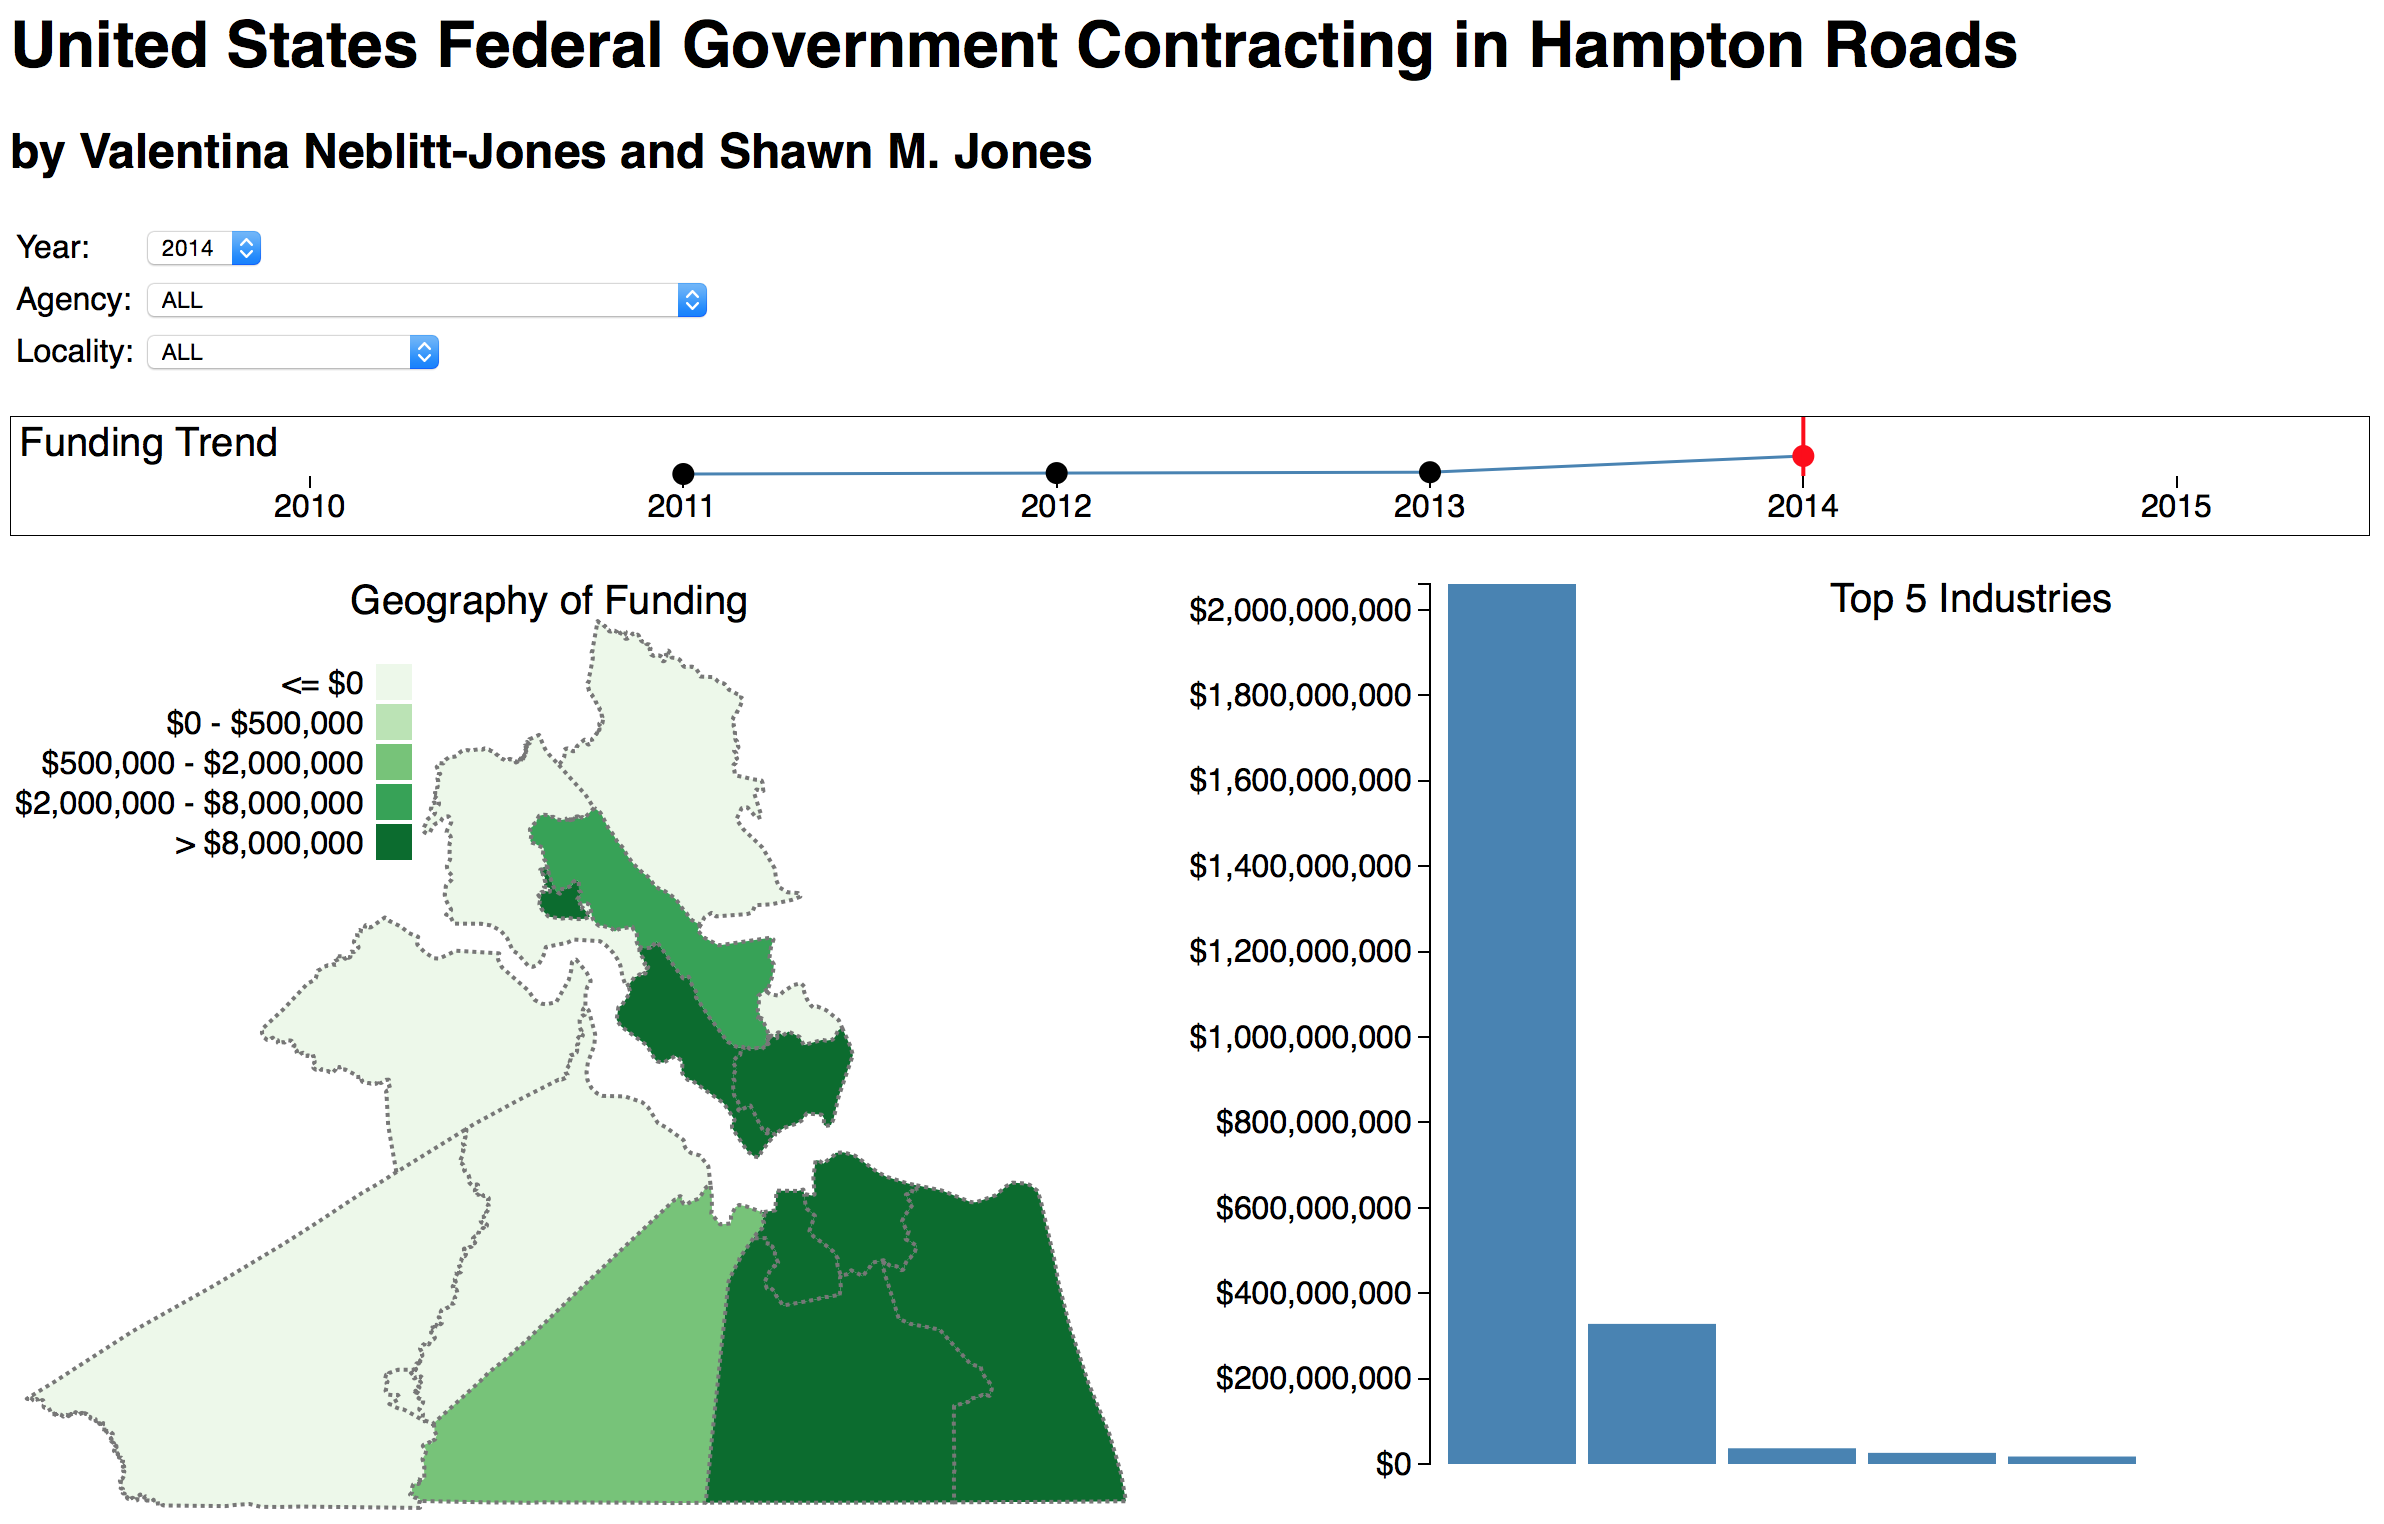
\includegraphics[width=0.45\textwidth]{images/teaser-screenie.png}
	\caption{The United States Federal Contracting in Hampton Roads visualization in its default state}
	\label{fig:default-main-vis}

	\vspace{3em}

	\centering
	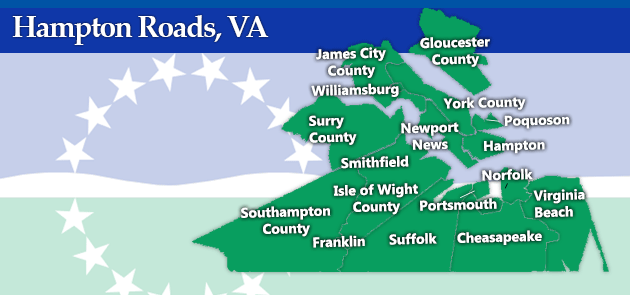
\includegraphics[width=0.4\textwidth]{images/HRFlagMapslide.png}
	\caption{Hampton Roads, as defined by the HRPDC}
	\label{fig:hrpdc-flag}
\end{figure}

Our region is Hampton Roads in the United States state of Virginia.  As defined by the Hampton Roads Planning District Commission (HRPDC), Hampton Roads consists of the City of Norfolk, the City of Virginia Beach, the City of Chesapeake, the City of Portsmouth, the City of Suffolk, the City of Franklin, Isle of Wight County, Southampton County, Town of Smithfield, Surry County, James City County, the City of Williamsburg, Gloucester County, York County, the City of Newport News, the City of Hampton, and the City of Poquoson.  Figure \ref{fig:hrpdc-flag} shows the map as defined by the HRPDC.  We use this definition of Hampton Roads in our visualization as well.

Existing visualizations of this data focus on the whole United States, or summarize data for types of funding.  We seek to create a visualization that is more specific to federal contracting in the Hampton Roads region, such that the Hampton Roads Planning District Commission can utilize the visualization for decision making.  We seek to help answer questions like the following:
\begin{itemize}
\item What industries are being funded in Hampton Roads?
\item What is the trend of funding in Hampton Roads (e.g. increasing, decreasing, stable)?
\item What knowledge areas should employees have to support work now and in the future in Hampton Roads?
\item What localities are receiving funding from which agencies?
\item How much funding does each locality receive from which agency?
\item Which agencies are providing funding to which industries in the region?
\end{itemize}

Using this visualization, we hope that the HRPDC can help guide decisions on such topics as funding for education and enticement for companies looking to move into the area. 

Others, however, have tried to visualize this data before.

\section{Related Work}

The \url{usaspending.gov} site does contain several ways to visualize the existing data.  These visualizations suffer from being too general for our needs, but we highlight them here in order to discuss for what they might be useful, and all of the ways in which they fail to meet our needs.  Each visualization appears on a different web page with separate controls, hence they are displayed separately.

Figure \ref{fig:existing-awards-by-year} shows the summary of awards for the current year, broken down into contracts, grants, loans, and other financial assistance.  It shows a bar chart, with each bar demonstrating the amount of money awarded for each category in the given year.  A user can generate a tooltip by hovering the mouse pointer over each bar.  This tooltip contains the value awarded for each award type, along with the number of transactions.  This visualization aggregates data for the whole United States, and does not break down the data for each locality in Hampton Roads.  We are also interested in contracting dollars, of which we are not interested.  It is also fixed to the current year, rather than allowing the user to select a given year to see the data.

Figure \ref{fig:existing-awards-by-state} shows the summary of awards for each state for the current year.  It is a choropleth coloring each state based on the amount of money awarded to each state.  Just like the bar chart, a user can generate a tooltip by hovering over each state.  This tooltip contains the value awarded to each state, along with the number of transactions.  This visualization provides data for a given state, such as Virginia, getting us closer to Hampton Roads, but it aggregates data of all types of awards; we are only interested in contracting data.  Just like the bar chart, it is fixed to the current year, not satisfying our need to see data from different years.

\begin{figure}[htbp]
	\centering
	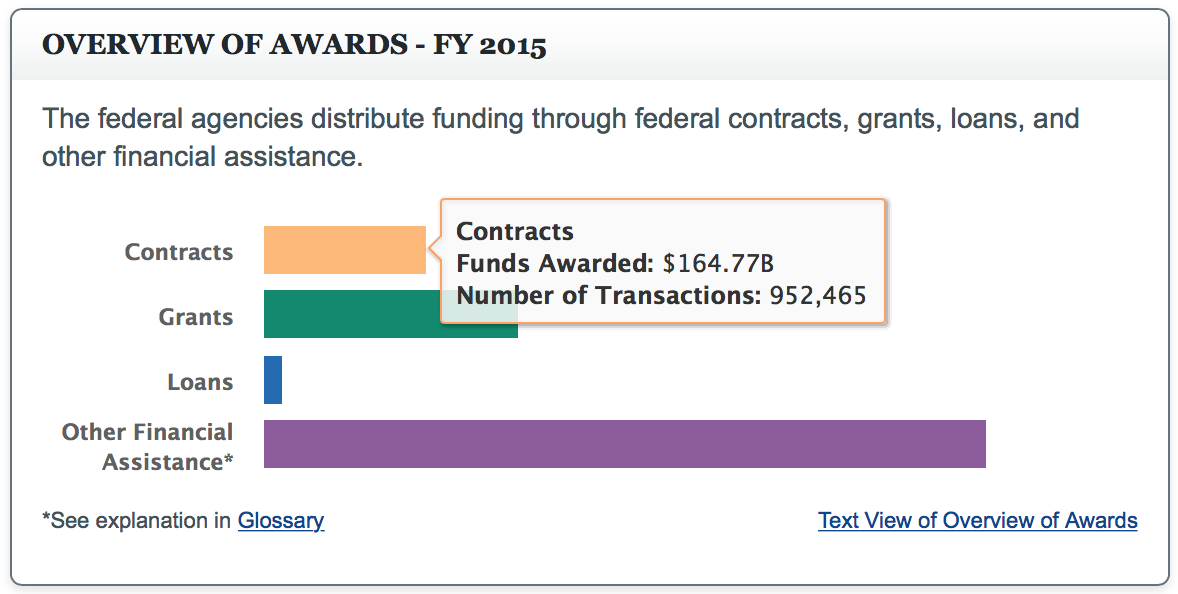
\includegraphics[width=0.5\textwidth]{images/existing-awards-by-year.png}
	\caption{USA Spending.gov visualization showing a summary of awards by year for the entire United States}
	\label{fig:existing-awards-by-year}

	\vspace{5em}

	\centering
	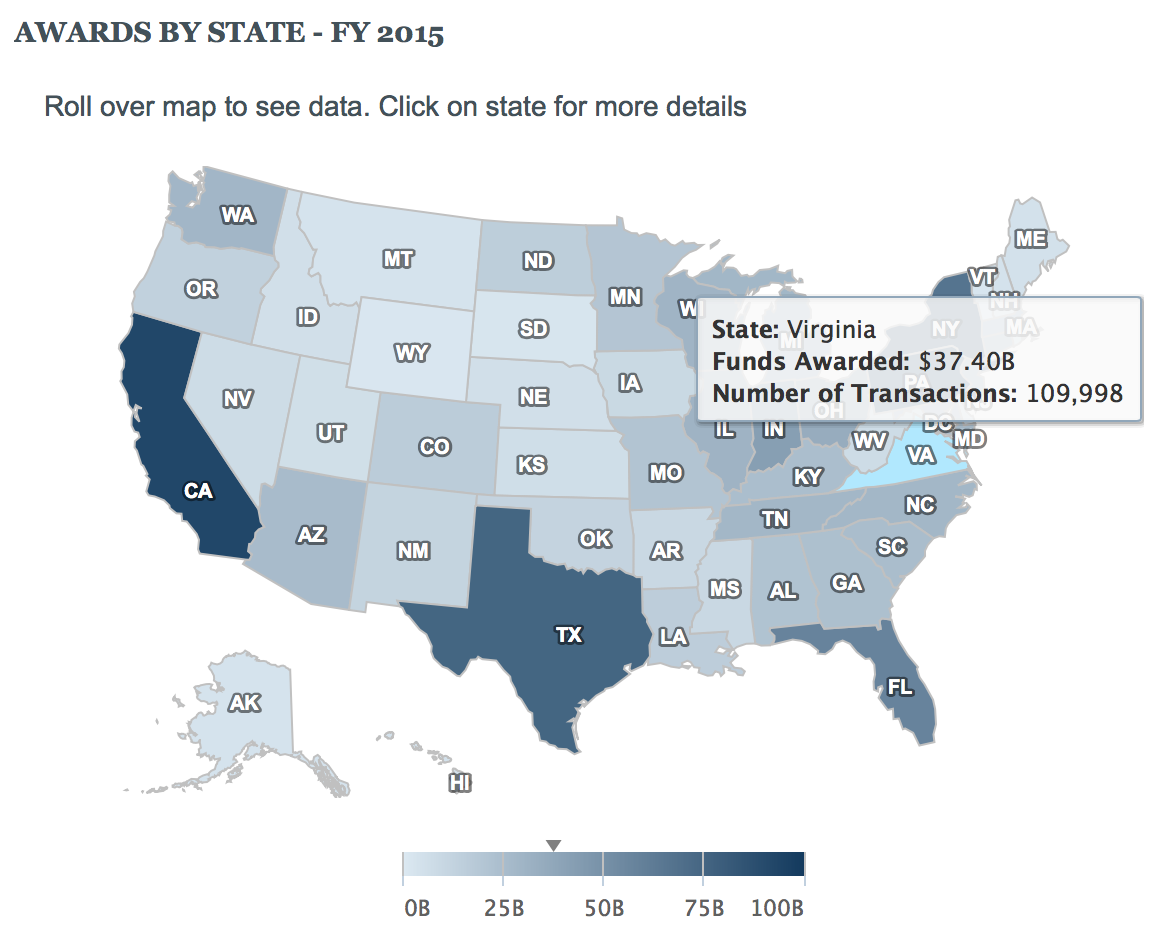
\includegraphics[width=0.5\textwidth]{images/existing-awards-by-state.png}
	\caption{USA Spending.gov visualization showing a summary of awards by state for the entire United States}
	\label{fig:existing-awards-by-state}

	\vspace{5em}

	\centering
	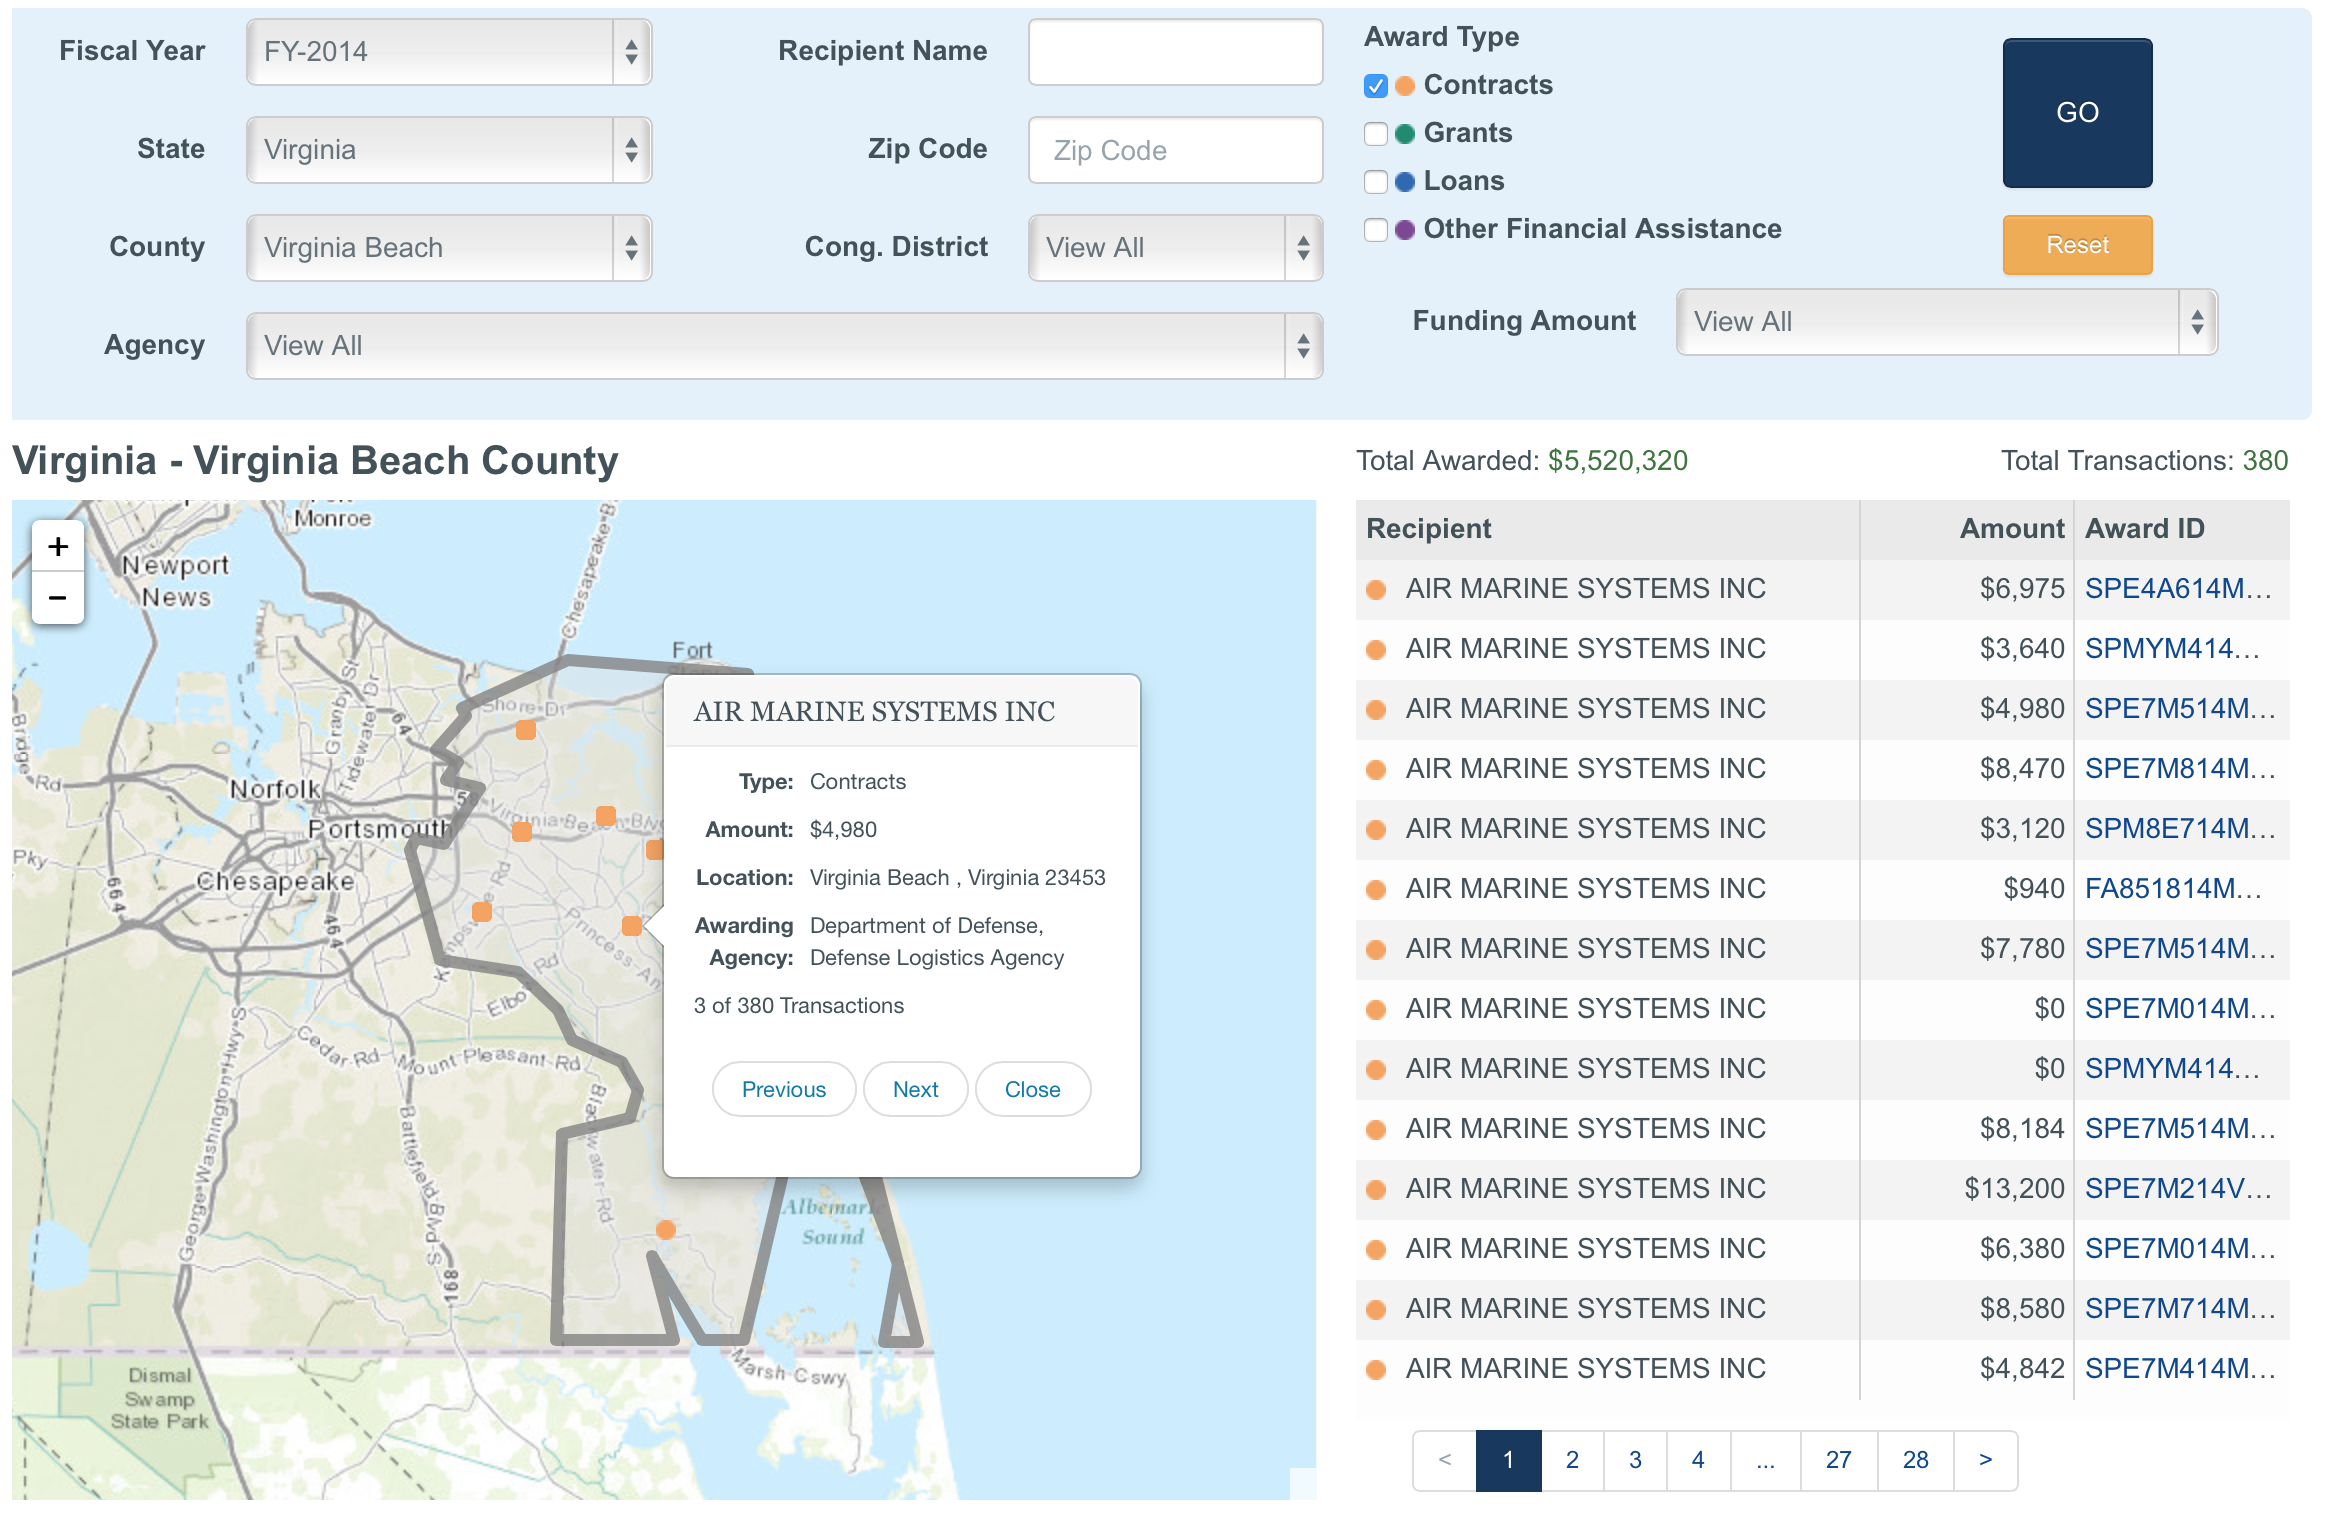
\includegraphics[width=0.5\textwidth]{images/existing-awards-by-locality.png}
	\caption{USA Spending.gov visualization showing a summary of awards by locality for the entire United States}
	\label{fig:existing-awards-by-locality}
\end{figure}

Figure \ref{fig:existing-awards-by-locality} is a more interactive visualization, providing data more in line with what we are looking for.  A user can use several drop down selectors to select the fiscal year, state, county, agency, ZIP code, congressional district, award type, amounth, and even restrict the the visualization to a specific recipient.  It provides information for the place of performance selected by the user, in this case the City of Virginia Beach.  It displays the contracts awarded to the right of the map, allowing the user to view each contract awarded.  The map provides squares pointing out where each contracting company is located.  A tooltip can be generated by the user by clicking on each square.  The tooltips contain information on the awarding agency, location, amount, and type of award.  This satisfies some of our needs, but does not contrast the different regions of Hampton Roads.  It also only displays information about prime award data, leaving out subcontractors, which are an important part of the work performed.  We also see no trend data, nor do we get industry data for comparison.

We want to show data for only Hampton Roads.  We also want to display industry information to address the questions we wished to answer with our visualization.  We want to allow the user to compare funding to individual localities based on agency and year.  Finally, we wanted to show trends across all years based on agency and locality.  The existing visualizations at \url{usaspending.gov} do not meet these needs.

\section{Data Processing}

Remember that our visualization consists of a choropleth, bar chart, and line chart.  Our data for this visualization comes from two sources.   The first source is \url{usaspending.gov}, providing the financial data for the visualization.  The second source is the United States Census geographic data site, from which we needed shapefiles for rendering the choropleth in our visualization.

\subsection{Financial Spending Data}

Data from \url{usaspending.gov} can be downloaded in CSV format using the form shown in Figure \ref{fig:data-download}.  Using this form, one can choose Prime or Sub Award data, the spending type (we wanted only contracts), the agency (we wanted all agency data), the fiscal year (we downloaded a single CSV for each year), the recipient state (we left this at all), place of performance state (we chose Virginia). select a date range (we left this at the default for the year selected), and chose the type of file to download (we chose CSV).

Not all data is available.  As shown in Figure \ref{fig:data-download-large-record-set}, some data combinations produced a download that could not be acquired via the web site.  Fortunately, we were only concerned with contracts where the work was performed in Virginia.  We tried to download data for Prime Award contracts in Virginia, but were told by the site that 0 records existed (in stark contrast to the results of their own visualizations), so we concentrated on Sub-Award data instead.

\begin{figure}[htbp]
	\centering
	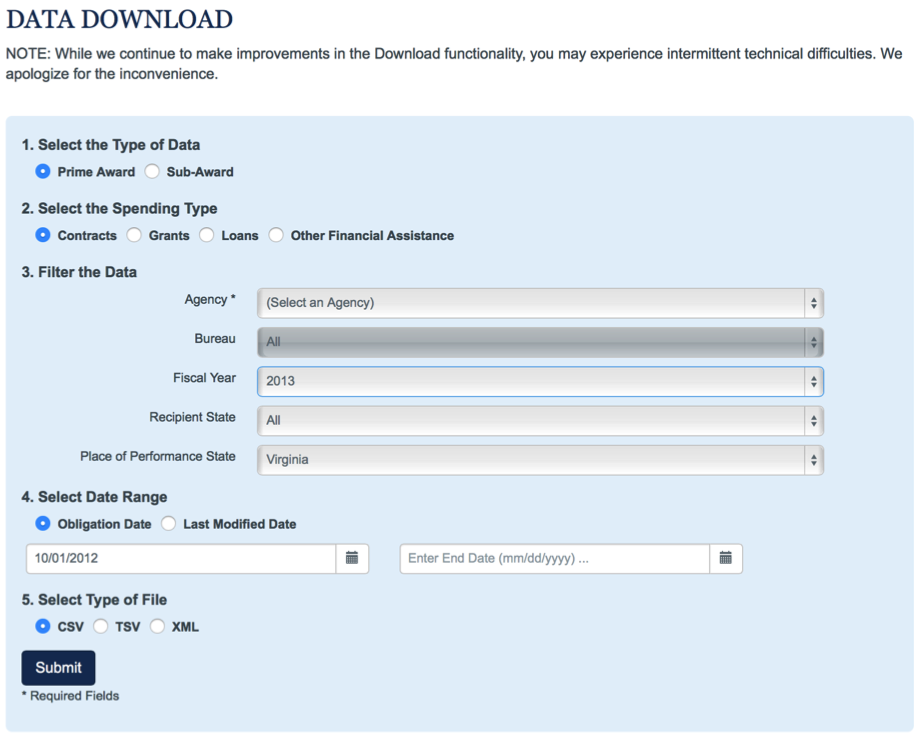
\includegraphics[width=0.4\textwidth]{images/data-download.png}
	\caption{For for downloading data from \protect\url{usaspending.gov}}
	\label{fig:data-download}
	
	\vspace{3em}
	
	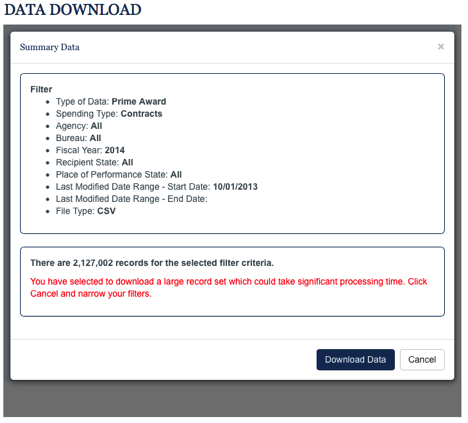
\includegraphics[width=0.4\textwidth]{images/data-download-large-record-set.png}
	\caption{Downloading large data sets is impossible via the web form at \protect\url{usaspending.gov}}
	\label{fig:data-download-large-record-set}

	\vspace{3em}

	\centering
	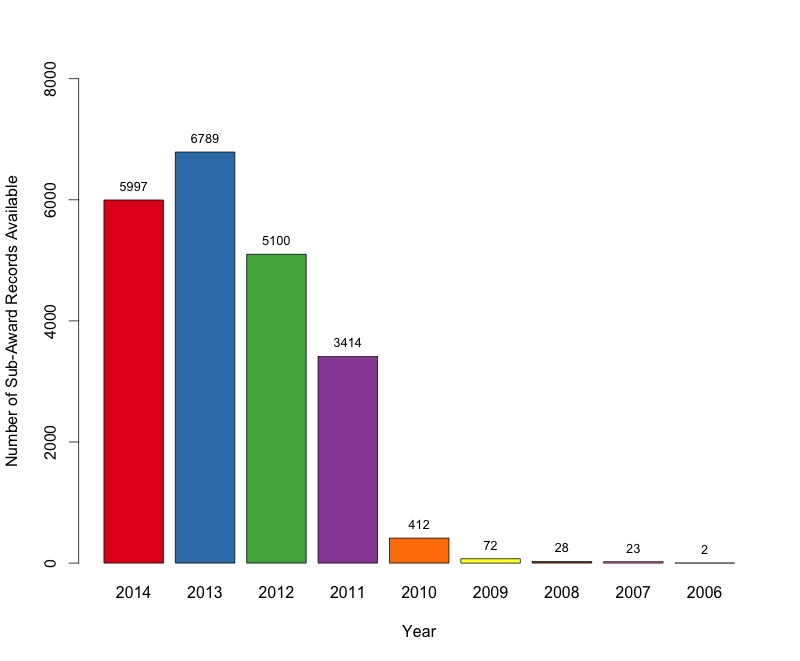
\includegraphics[width=0.4\textwidth]{images/numrecords-barplot.png}
	\caption{Number of Sub-Award records available from \protect\url{usaspending.gov} for Virginia for each year; note the precipitous falloff prior to 2011}
	\label{fig:numrecords-barplot}	
\end{figure}

We downloaded the data for years 2006 - 2014 on April 1, 2015.  Being relegated to Sub-Award data, we attempted to download records for all of the years available.  We found that the number of records decreases precipitously, as shown in Figure \ref{fig:numrecords-barplot}.  For example, we found it hard to believe that the entire state of Virginia only had 2 contracts awarded in 2006.  These outliers forced us to consider any data from 2006 - 2010 as suspect, so we limited the year range of the data to only 2010 - 2014, ensuring that our visualization would feature the most accurate data we could find.

The CSV files consisted of 101 fields, providing information on each contract awarded.  From these files, and also using the provided data dictionary, we identified five useful fields for our endeavor.  Table \ref{tab:data-mapping} lists these fields and how we mapped them during our data processing.  We use the {\tt subaward\_principle\_place\_city} field to indicate the locality in which the work took place.  We use the {\tt subaward\_principle\_naics\_desc} field for information on which industry the contract applies to.  We use the {\tt subaward\_major\_agency\_name} field to identify the agency each contract applies to.  Contracts are complex, and have many pieces.  We had 3 agency fields to choose from, but {\tt subaward\_major\_agency\_name} indicates funding for the particular subcontractor performing work in the region, not necessarily the agency that controls the overall contract across the United States.  We use {\tt subaward\_amount} to indicate the amount of funding for the contract.  We chose this rather than the prime award amount because we are only interested in funding that ends up in Hampton Roads.  We use {\tt subaward\_fiscal\_year} to determine which data ends up in our visualization for a given year.  Most of the time, this field matched the download, but there were a few cases where it failed to, meaning that the subaward was dispersed in a separate year than the contract was awarded.  We were concerned about when the money ended up in Hampton Roads, so we use this field to ensure the data is correct.

Once we had acquired the CSV files, we then needed to clean the data and ensure that it only contained records for Hampton Roads.  For this step we used OpenRefine, as shown in Figure \ref{fig:openRefine-2014-data}.  OpenRefine allowed us to correct the many spelling mistakes present for each entry in the {\tt subaward\_principle\_place\_city} field.  It also allowed us to standardize capitalization for the different localities.  Oddly, as one can see in Figure \ref{fig:openRefine-2014-data}, the data contained addresses in this city field.  We had to use resources, such as Google Maps, to identify which localities these addresses corresponded to.  Thanks to this step, we were able to include more data about contracting in the region that would have been left out if we had just honored the existing city entries.  Also, the file contained cities that do not exist in Virginia, such as San Diego, even though we requested a data download only containing records for Virginia.  To resolve these inconsistencies, we used the {\tt subaward\_principle\_place\_zip} field to determine if the ZIP code is in Virginia, and, more importantly in Hampton Roads.  The {\tt subaward\_federal\_agency\_name} field appeared to have a controlled vocabulary, but we converted the agency names so that they would support consistency throughout the visualization; for example, ``DEPT OF DEFENSE'' was changed ``Dept of Defense, but also listed was ``COMMERCE, DEPARTMENT OF'', which we changed to ``Dept of Commerce'' for consistency of nomenclature for sorting and viewing.  We left the controlled vocabulary field of {\tt subaward\_principle\_naics\_city} alone, seeing as we required no consistency from its values for our bar chart.


\begin{figure}[htbp]
	\centering
	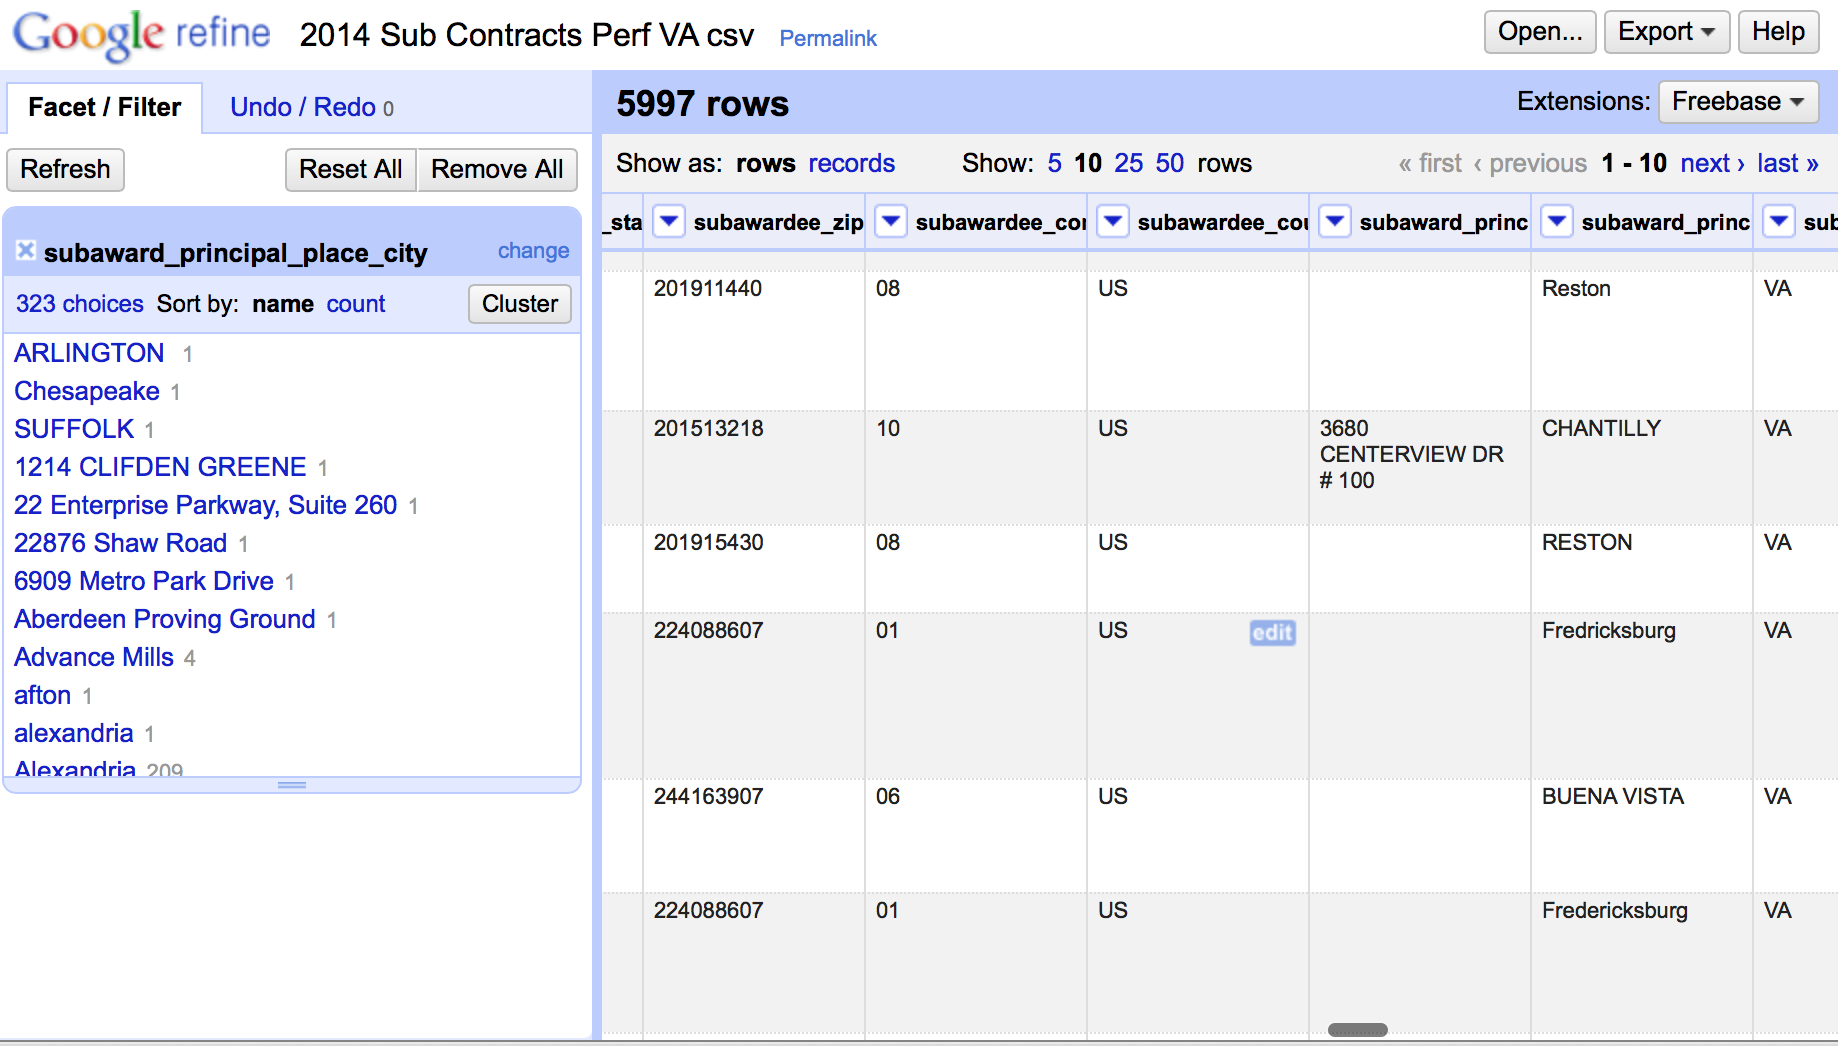
\includegraphics[width=0.5\textwidth]{images/openRefine-2014-data.png}
	\caption{Data from \protect\url{usaspending.gov} loaded into OpenRefine (formerly Google Refine)}
	\label{fig:openRefine-2014-data}	

	\vspace{3em}

	\centering
	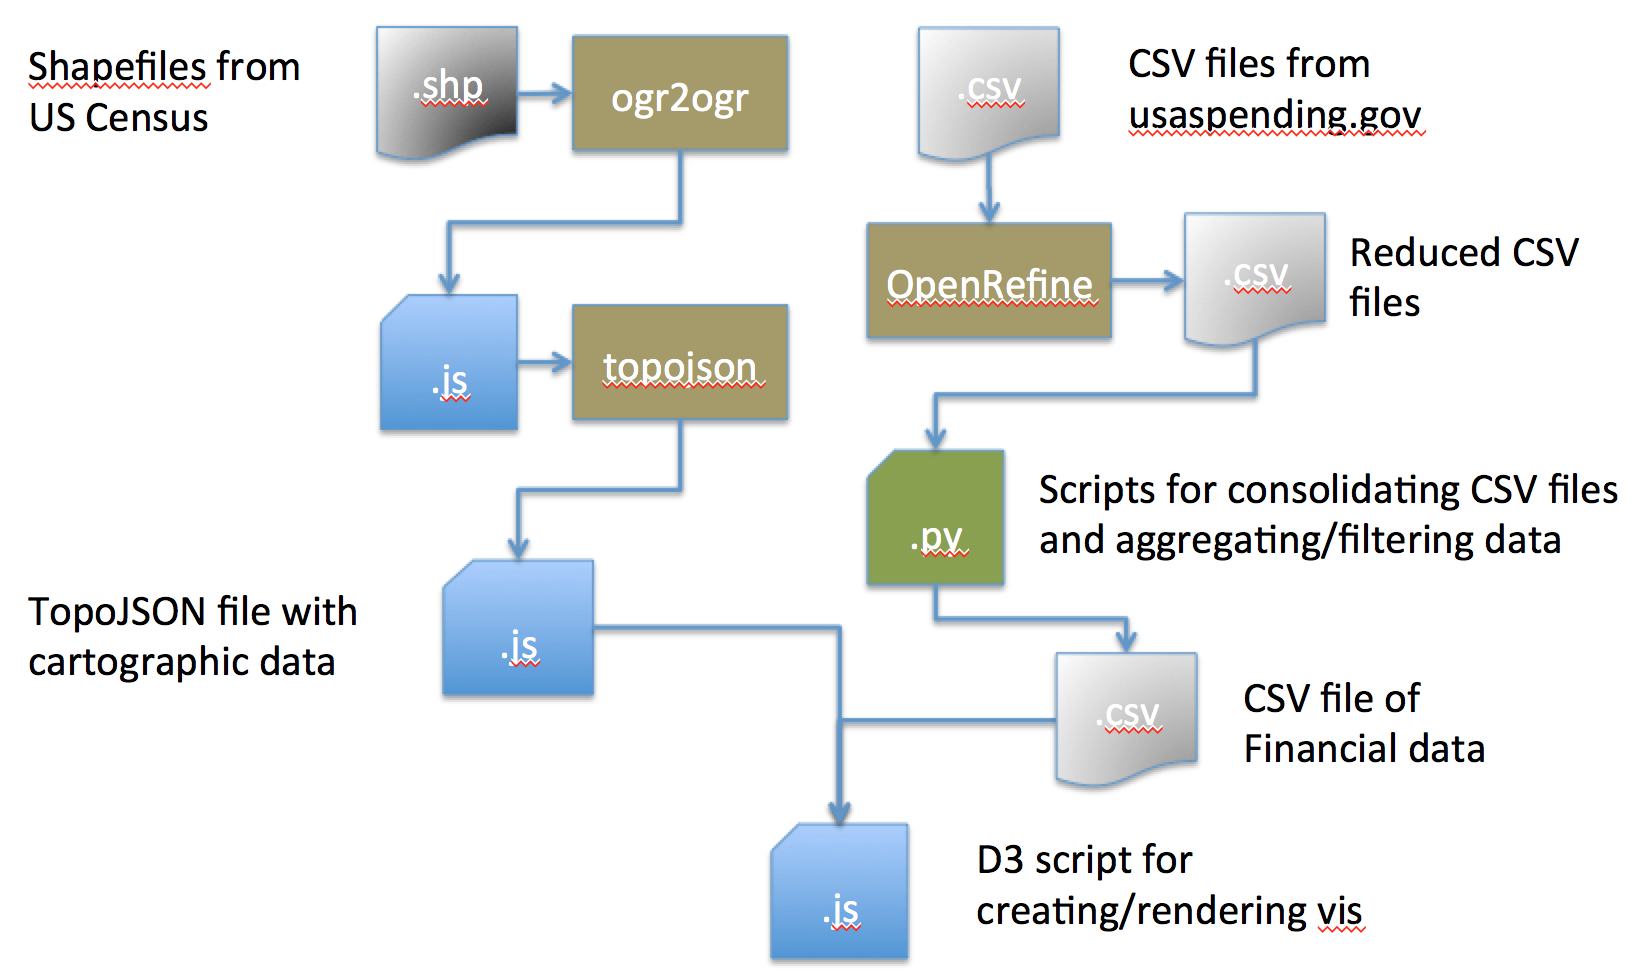
\includegraphics[width=0.5\textwidth]{images/data-flow.png}
	\caption{Data flow to produce CSV and JSON map data for visualization}
	\label{fig:data-flow}	
\end{figure}

\begin{table}[t]
\centering
\begin{tabular}{l | l}
\hline
\textbf{Original field name} & \textbf{Field Name} \\
\textbf{from usaspending.gov} & \textbf{for our visualization} \\ \hline
subaward\_principal\_place\_city         & locality                         \\
subaward\_principal\_naics\_desc         & industry                         \\
subaward\_federal\_agency\_name          & agency                           \\
subaward\_amount                         & funding                          \\
subaward\_fiscal\_year                   & year                                 \\ \hline
\end{tabular}
\caption{Mapping of fields from \protect\url{usaspending.gov} into fields useful for our visualization}
\label{tab:data-mapping}
\end{table}

Once we had cleaned CSV files for each year, we then used a Python script, as shown in Figure  to compute all possible combinations of Agency, Year, and Locality, summing up the funding amounts for each.  The Python script calculates every combination of choice, and uses the value ``ALL'' in a field to assist in generating the data for each part of our visualization.  Table \ref{tab:use-of-all} shows how the use of ``ALL'' in individual fields results in aggregated values and which part of the visualization to which they pertain.

\begin{table}[t]
\centering
\begin{tabular}{l | l | l}
\textbf{``ALL''} & \textbf{Available User} & \textbf{Part} \\
\textbf{in field} & \textbf{Selections} & \textbf{of Vis} \\
\hline
none & locality, agency, & Industry Bar Chart \\
& year & for specific industries \\
\hline
industry & locality, agency, & Choropleth for user \\
& year & selection, including values \\
& & for all industries;  \\
& & also Sparkline \\
& & for user selection \\
\hline
locality & agency, year & Industry Bar Chart \\
& & for all localities \\
\hline
agency & locality, year & Industry Bar Chart \\
& & for all agencies \\
\hline
agency, locality & year & Industry Bar Chart \\
& & for all localities and agencies \\
\hline
agency, locality, & year & Sparkline \\
industry &  & for all localities and agencies \\
\hline
locality, industry & year, agency & Sparkline \\
& & for all localities, \\
& & but selected agency \\
\hline
agency, industry & year, locality & Sparkline \\
& & for single locality, \\
& & all agencies \\
\hline
\end{tabular}

\caption{Use of the ``ALL'' value in various fields allows our vis to aggregate data for different combinations of user selections}
\label{tab:use-of-all}

\end{table} 




\subsection{Geographic Data}

\section{Our Visualization}

\section{Conclusion}


\section{Final Thoughts}


\appendices
\section{Proof of the First Zonklar Equation}
Appendix one text goes here.

% you can choose not to have a title for an appendix
% if you want by leaving the argument blank
\section{}
Appendix two text goes here.


% use section* for acknowledgment
\ifCLASSOPTIONcompsoc
  % The Computer Society usually uses the plural form
  \section*{Acknowledgments}
\else
  % regular IEEE prefers the singular form
  \section*{Acknowledgment}
\fi


The authors would like to thank...


% Can use something like this to put references on a page
% by themselves when using endfloat and the captionsoff option.
\ifCLASSOPTIONcaptionsoff
  \newpage
\fi



% trigger a \newpage just before the given reference
% number - used to balance the columns on the last page
% adjust value as needed - may need to be readjusted if
% the document is modified later
%\IEEEtriggeratref{8}
% The "triggered" command can be changed if desired:
%\IEEEtriggercmd{\enlargethispage{-5in}}

% references section

% can use a bibliography generated by BibTeX as a .bbl file
% BibTeX documentation can be easily obtained at:
% http://www.ctan.org/tex-archive/biblio/bibtex/contrib/doc/
% The IEEEtran BibTeX style support page is at:
% http://www.michaelshell.org/tex/ieeetran/bibtex/
%\bibliographystyle{IEEEtran}
% argument is your BibTeX string definitions and bibliography database(s)
%\bibliography{IEEEabrv,../bib/paper}
%
% <OR> manually copy in the resultant .bbl file
% set second argument of \begin to the number of references
% (used to reserve space for the reference number labels box)
\begin{thebibliography}{1}

\bibitem{IEEEhowto:kopka}
H.~Kopka and P.~W. Daly, \emph{A Guide to {\LaTeX}}, 3rd~ed.\hskip 1em plus
  0.5em minus 0.4em\relax Harlow, England: Addison-Wesley, 1999.

\end{thebibliography}

% biography section
% 
% If you have an EPS/PDF photo (graphicx package needed) extra braces are
% needed around the contents of the optional argument to biography to prevent
% the LaTeX parser from getting confused when it sees the complicated
% \includegraphics command within an optional argument. (You could create
% your own custom macro containing the \includegraphics command to make things
% simpler here.)
%\begin{IEEEbiography}[{\includegraphics[width=1in,height=1.25in,clip,keepaspectratio]{mshell}}]{Michael Shell}
% or if you just want to reserve a space for a photo:

%\begin{IEEEbiography}{Shawn M. Jones}
%Biography text here.
%\end{IEEEbiography}

% if you will not have a photo at all:
\begin{IEEEbiographynophoto}{Shawn M. Jones}
is a computer scientist with Space and Naval Warfare Systems Center Atlantic in Norfolk, VA. He completed his B.S. and M.S. in computer science from Old Dominion University. He is a Ph.D. student in computer science at Old Dominion University.
\end{IEEEbiographynophoto}

% insert where needed to balance the two columns on the last page with
% biographies
%\newpage

\begin{IEEEbiographynophoto}{Valentina Neblitt-Jones}
is the Head of Systems Development at Old Dominion University Libraries in Norfolk, VA. She completed her B.A. in international studies at Virginia Tech, B.S. in computer science at Old Dominion University, and M.S in library science at Florida State University.
\end{IEEEbiographynophoto}

% You can push biographies down or up by placing
% a \vfill before or after them. The appropriate
% use of \vfill depends on what kind of text is
% on the last page and whether or not the columns
% are being equalized.

%\vfill

% Can be used to pull up biographies so that the bottom of the last one
% is flush with the other column.
%\enlargethispage{-5in}



% that's all folks
\end{document}


